% based on Msc dissertation template of University of Edinburgh

\documentclass[msc,deptreport, cs]{infthesis}
\usepackage{subfig} 
\graphicspath{{figures/}}

\begin{document}
\begin{preliminary}

\title{Developing an Application \\to Introduce Parallel \\Task Scheduling}

\author{Juntong Liu}

\abstract{
}

\maketitle

\section*{Acknowledgements}
Any acknowledgements go here. 

\tableofcontents
\end{preliminary}


\chapter{Introduction}

Computing resource is in high demand both in industry and for academic research. In industry, companies are collecting terabytes or even petabytes of user data to provide customized services. Also, machine learning algorithms are widely used to provide suggestions and to extract information from media files. Processing these files and executing these algorithms all requires numerous amount of computing resource. In academic research, many researchers in subjects like hydromechanics and electrics rely on simulation to predict the performance of models. In this case, more computing resource is consumed for better resolution.

However, researchers said Moore's Law will not be effective in the near future (ref), meaning speed of improvement in single core performance may be far behind the increasing demand. Therefore, the typical way to utilize more computing resource is to use multiple processors to work on the same task in parallel. Traditional code for single code execution cannot be used directly for parallel execution. They have to be modified. One common solution to parallelize a big task is to divide them into small tasks that can be executed separately on multiple processors. However, in most of cases, the small tasks cannot be independent because they might require data produced by other tasks. The dependency can be usually represented by a DAG (directed acyclic graph) called task graph.

In large-scaled systems, tasks in a task graph are managed and scheduled to processors by a scheduler dynamically based on certain scheduling algorithm. To have better understanding of task graph scheduling, students need to learn the algorithms. However, learning such algorithms are not easy for many students for several reasons:

\begin{itemize}
  \item There are many models to describe the behavior of processors in real life. Students can be confused by the variety.
  \item Algorithms are usually given based on a certain model. For other models, there might be many variants that are slightly different, making things more confusing.
  \item Task scheduling requires predicting states of the cluster for a long duration. This is hard because it requires good imagination and detailed understanding of the behavior of models.
  \item Some algorithms requires sophisticated control over the timeline, or have complex mathematical model which is hard to understand.
\end{itemize}

This project aims to develop an game-like application to help the students learn concepts in task graph scheduling, in addition to algorithms. For any schedule, it can simulate the execution timeline based on a variety of cluster configurations. It also provides a step to step tutorial to help students learn the mechanisms and algorithms. For tutors, this application can also be used for demonstration.

\chapter{Background}

\section{Task Graph Scheduling}

\begin{figure}[htpb]
  \centering
  \subfloat[task graph]{ 
      \label{fig:graph}
      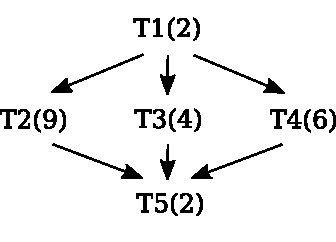
\includegraphics[width=0.3\columnwidth]{graph.pdf}
  } \hspace{2em}
  \subfloat[schedule]{
      \label{fig:schedule}
      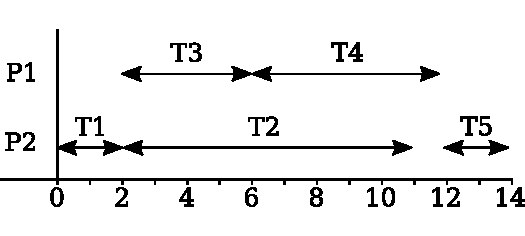
\includegraphics[width=0.45\columnwidth]{schedule.pdf}
  }
  \caption{Example of task graph and one possible schedule}
  \label{fig:example}
\end{figure}

The topic of this project is task graph scheduling. Figure \ref{fig:graph} shows an example task graph.

\subsection{Different Models}

\subsection{HLEFT Algorithm}

\section{Educational Software}

\chapter{Methodology}

\section{Learning Experience}

\section{Design of Interface}

\section{Platform and Libraries}

\subsection{Programming Language}

This project is designed to be a cross-platform desktop application. While C++ is the typical choice for such requirements, Java is chosen as the main language in development. 

The biggest difficulty of using C++ is compilation on different platforms. For example, programs on Windows are usually compiled against all DLLs (dynamically linked libraries) selected and provided by the developer and distributed with all its dependencies bundled. However on Linux, programs are usually compiled against SOs (shared objects) provided by system, then distributed as source file or single binary file. Such difference brings complexity in compilation and potential issues in distribution.

Oppositely, compilation of Java file is much easier. With help of virtual machine, compiled binary files can be executed on different platforms without any extra step. Since Java executable files are usually packed in Jar files, distribution is also convenient.

\subsection{GUI Library}

As is said in previous sections, the interface is designed to be interactive, which means the application will heavily rely on operations like hovering and drag \& drop. Also, it requires rendering overlays and transparency frequently. For widgets based traditional GUI frameworks, these operations usually requires usage of complex or low level APIs, which brings difficulty in development and potential compatibility issues. Therefore, games are usually developed based on dedicated GUI frameworks.

GUI frameworks used in games are usually built on low level libraries like DirectX and OpenGL. One reason is they are usually directly connected to hardware operations, which saves much performance in rendering complex shapes. Another reason is these libraries allows GUI frameworks developed in immediate mode, making it easier to develop highly dynamic scenes. Compared to retained mode, the developer do not need to refresh windows manually in immediate mode because every frame is refreshed and rendered separately.

OpenGL is chosen as the rendering library for its cross-platform availability and simplicity. Although OpenGL do not provide APIs in Java, there are several libraries in Java providing the bridge. Among these libraries, LWJGL 3 is chosen for several reasons:

\begin{itemize}
  \vspace{-1em}\item It includes bridges to several convenient native libraries like STB and GLFW.
  \vspace{-1em}\item It has very good documents and community support.
  \vspace{-1em}\item It provides full exposure of OpenGL APIs.
  \vspace{-1em}\item It it up-to-date.
\end{itemize}


\chapter{Implementation}

\section{Simulation Engine}

\subsection{Communication Models}

\subsection{Processor Model}

\section{GUI Framework}

\subsection{Rendering Method}

\subsection{Widgets and Layout}

\section{Data Driven Format}

\section{Algorithms and Estimator}

\section{Event System}

\subsection{Tutorials}

\chapter{Result}

\section{Compilation and Distribution}

\section{Game Flow}

\subsection{Tutorial Levels}

\subsection{Game Levels}

\section{Sandbox Mode}

\chapter{Evaluation}

\section{User Testing}

\section{Code Quality}

\chapter{Conclusions}

\section{Future Suggestions}

\section{Final Comments}

\bibliographystyle{plain}
\bibliography{main}

\end{document}
